\documentclass[a4paper, 12pt, titlepage]{scrartcl}

\usepackage[utf8]{inputenc}
\usepackage[T1]{fontenc}
\usepackage{mathptmx}
\fontfamily{ptm}

\usepackage[ngerman]{babel}
\babelhyphenation[ngerman]{Re-in-fek-tion}
\usepackage{csquotes}

\usepackage{setspace}
\onehalfspacing
\usepackage[top=3cm, bottom=3cm, left=4cm, right=4cm]{geometry}

\usepackage{amsmath,amssymb,amstext, mathtools}
\usepackage{tabularx}
\renewcommand{\arraystretch}{1.5}

\usepackage{pdfpages}
\usepackage{subfiles}

\usepackage{tikz}
\usetikzlibrary{math}
\usetikzlibrary{arrows, arrows.meta}

\usepackage{graphicx}
\graphicspath{{figures/}}

\usepackage[style=alphabetic, sorting=nty, backend=biber]{biblatex}
\addbibresource{ref.bib}
\DeclareDelimFormat[bib]{nametitledelim}{\addcolon\space}
\DeclareNameAlias{default}{family-given}
\DefineBibliographyStrings{ngerman}{
  andothers = {et\addabbrvspace al\adddot}
}

\usepackage{xurl}
\usepackage{microtype}

\usepackage{xcolor}
\definecolor{codepink}{rgb}{0.6, 0,   0.8}
\definecolor{codeblue}{rgb}{0.9, 0.2, 0.4}
\definecolor{codegray}{rgb}{0.5, 0.5, 0.5}
\definecolor{codeback}{rgb}{1, 1, 0.9}

\usepackage{listings}
\lstset{ 
  language=Python,
  backgroundcolor=\color{codeback},
  keywordstyle=\color{codepink},
  stringstyle=\color{codeblue},
  commentstyle=\color{codegray},
  numberstyle=\small\color{codegray},
  basicstyle=\ttfamily\footnotesize,
  breaklines=true,
  breakatwhitespace=false,
  keepspaces=true,
  numbers=left,
  showspaces=false,
  showstringspaces=false,
  showtabs=false,
  tabsize=2,
  literate=
  {Ö}{{\"O}}1 
  {Ä}{{\"A}}1 
  {Ü}{{\"U}}1 
  {ß}{{\ss}}1 
  {ü}{{\"u}}1 
  {ä}{{\"a}}1 
  {ö}{{\"o}}1 
  {~}{{\textasciitilde}}1 
} 

\newcommand{\Title}{Untersuchung der weiteren Entwicklung von Covid-19 in Deutschland}
\newcommand{\Subject}{Erweiterung des SIR-Modells um Immunitätsverlust, Impfungen und Saisonalität}
\newcommand{\Author}{Samuel Mulzer}

\usepackage{hyperref}
\hypersetup{
  pdftitle    = {\Title},
  pdfsubject  = {\Subject},
  pdfauthor   = {\Author},
  pdfkeywords = {Covid-19, Deutschland} ,
  pdfcreator  = {latexmk},
  pdfproducer = {LaTeX with hyperref},
  colorlinks  = true,
  linkcolor   = black,
  citecolor   = black,
  urlcolor    = blue,
  filecolor   = magenta
}

\title{\Title}
\subtitle{\Subject}
\author{\Author}
\date{8. November 2022}

\begin{document}
  \maketitle
  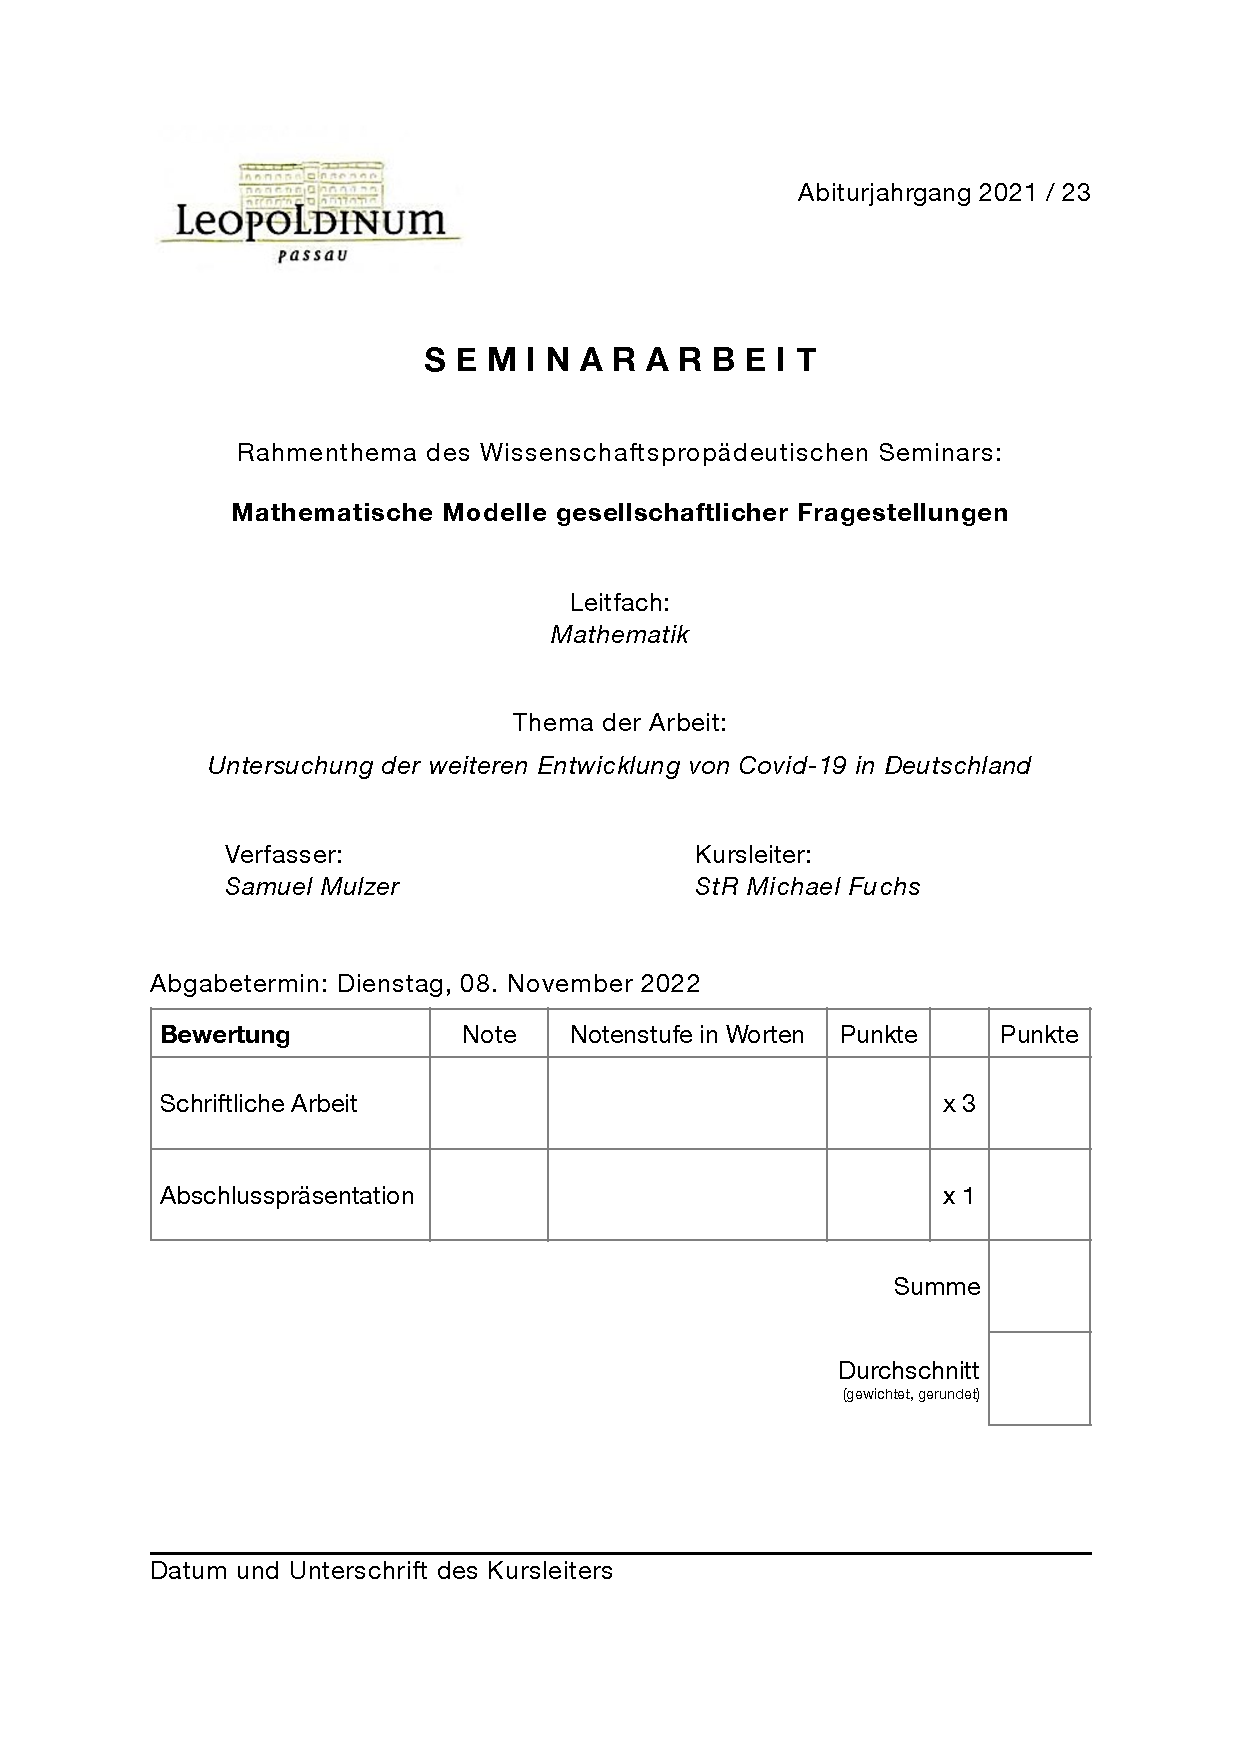
\includepdf{sections/cover}

  \renewcommand{\contentsname}{Inhaltsverzeichnis}
  \thispagestyle{empty}
  \tableofcontents
  \clearpage
  \newpage

  \setcounter{page}{3}

  \section*{Einführung}
  \label{sec:introduction}
  \addcontentsline{toc}{section}{Einführung}
  \subfile{sections/introduction}
  \newpage

  \section{Das Anwendungsproblem}
  \label{sec:problem}
  \subfile{sections/problem}
  \newpage
  
  \section{Das klassische SIR-Modell}
  \label{sec:basic_model}
  \subfile{sections/basic_model}
  \newpage

  \section{Das erweiterte Modell}
  \label{sec:extended_model}
  \subfile{sections/extended_model}
  \newpage

  \section*{Fazit}
  \label{sec:conclusion}
  \addcontentsline{toc}{section}{Fazit}
  \subfile{sections/conclusion.tex}
  \newpage


  \addcontentsline{toc}{section}{Literaturverzeichnis}
  \renewcommand{\refname}{Literaturverzeichnis}
  \printbibliography
  \newpage

  \addcontentsline{toc}{section}{Abbildungsverzeichnis}
  \renewcommand{\listfigurename}{Abbildungsverzeichnis}
  \listoffigures
  \bigskip
  Alle Abbildungen wurden selbstständig erstellt.
  \newpage

  \section*{Anhang}
  \label{sec:appendix}
  \addcontentsline{toc}{section}{Anhang}
  \subfile{sections/appendix}
  \newpage

  \section*{Eigenständigkeitserklärung}
  Ich erkläre, dass ich die Seminararbeit ohne fremde Hilfe angefertigt und nur die im Literaturverzeichnis angeführten Hilfsmittel verwendet habe. \\[0.3cm]
  Passau, den 8. November 2022 \\[2cm]
  \rule{6cm}{.4pt} \\
  Samuel Mulzer

\end{document}
